\section{Alignment and response-error checks}\label{app:approximate-feedback}
For the normal space $K=\operatorname{span}(e_1,e_2,e_3)$, set
$g=(e_1+e_2+e_3)/\sqrt3$,
$h_1=(e_1-e_2)/\sqrt2$ and $h_2=(e_1+e_2-2e_3)/\sqrt6$.
The perturbed embedding is
\begin{equation}
 P_\theta=[g,\cos\theta e_4+\sin\theta h_1,
                 \cos\theta e_5+\sin\theta h_2,e_6]H.
\end{equation}
Its nonzero candidate singular values are $(1,\sin\theta,\sin\theta)$.
Exact rank is one at zero and three for every tested $\theta>0$.
Angles are $0$, $10^{-6}$, $10^{-4}$, $0.01$, $0.1$ and $0.5$ radians.
We use one or three queries, response-error norms $0,10^{-6},10^{-3}$, and 64 constructed
normals per cell. Negative normals of norm one on the first three
coordinates, with target $(0.5,0.5,0.5,0,\ldots,0)$, define compatible
quadratics through $b=n-2av$. Feasible queries use $\alpha=0.25$.

All 2,304 checks satisfy Eq.~\eqref{eq:truncated-feedback} and its
cost-difference bound. For one noiseless query the bound is
$\sin\theta$; response noise adds orthogonally. Figure~\ref{fig:approximate-feedback}
shows the observed maxima. These are algebraic checks with known
$M=1$, not noisy-network training or evidence that arbitrary perturbations
preserve the one-query exact result. The neural implementation's Gram
eigenvalue threshold $10^{-10}$ would discard sufficiently small positive
singular values; the perturbed checks use the explicit spectrum above.
\begin{figure}[htbp]\centering
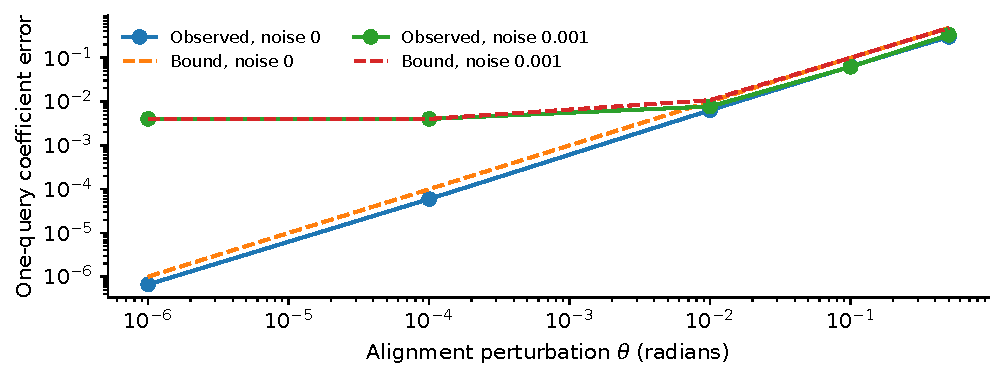
\includegraphics[width=.88\linewidth]{figures/approximate_feedback.pdf}
\caption{One-query error under perturbed alignment. Points show maxima
over 64 compatible normals per cell; dashed curves give the upper bound.}
\label{fig:approximate-feedback}
\end{figure}
